\documentclass[12pt]{article}
\usepackage[utf8]{inputenc}
\usepackage[a4paper, margin=1.5cm]{geometry}
\usepackage{multicol}
\usepackage[portuguese]{babel}
\usepackage{hyperref}
\usepackage{xurl}
\usepackage{graphicx}
\usepackage{tabularx}
\usepackage{wrapfig}
\usepackage{float}
\graphicspath{ {./img/} }

%%%%%%%%%%%%%%%%%%%%%%%%%%%%%%%%%%%%%%%%%%%%%%%%
%%%%%%%%%%%%%%%%%%%%%%%%%%%%%%%%%%%%%%%%%%%%%%%%
%%%%%%%%%%%%%%%%%%%%%%%%%%%%%%%%%%%%%%%%%%%%%%%%

\title{Convite aos colegas para novo grupo de estudo na UFCA}
\author{Thyago Ismael}
\date{\today}

\begin{document}
\maketitle

\begin{abstract}
    É comum ver nos cursos de Ciência da Computação e afins alunos se preocupando com qual linguagem de programação ou ferramenta de desenvolvimento escolher para estudar, uma vez que isso demanda tempo e, frente a um mercado em rápida evolução, receiam ficar para trás. Na tentativa de ajuda-los, este texto propõe a criação de um ambiente de estudos dentro da instituição no qual se pode conhecer e experimentar mais uma das áreas disponíveis no mercado a partir do desenvolvimento de projetos internos nos modelos comerciais. Além disso, detalha-se um projeto inicial que combina duas áreas em franco crescimento na intenção de permitir a interessados em uma conhecer sobre a outra.
\end{abstract}
\vspace{24pt}


%%%%%%%%%%%%%%%%%%%%%%%%%%%%%%%%%%%%%%%%%%%%%%%%%%%%%%%%%%%%%%%%%%%%%%%%%%%%%%%%%%%%%%%%%%%%%%%%
%%%%%%%%%%%%%%%%%%%%%%%%%%%%%%%%%%%%%%%%%%%%%%%%%%%%%%%%%%%%%%%%%%%%%%%%%%%%%%%%%%%%%%%%%%%%%%%%
%%%%%%%%%%%%%%%%%%%%%%%%%%%%%%%%%%%%%%%%%%%%%%%%%%%%%%%%%%%%%%%%%%%%%%%%%%%%%%%%%%%%%%%%%%%%%%%%


\section{Introdução}
\begin{multicols}{2}
    Tão logo o semestre letivo se inicia, é possível ouvir sobre os principais tópicos da Ciência e da Engenharia da Computação pelos corredores do campus. Ouve-se sobre as implicações psico-metafísicas da computação quântica na geopolítica aplicada, sobre as últimas inovações na corrida espacial, sobre o impacto da tecnologia embutida no subconsciente humano, etc. Tudo no primeiro dia. No entanto, não demora muito para o recém-ingresso perceber que o mundo ao seu redor difere sobremaneira do virtual, no qual o entretenimento, não a veracidade técnica ou aplicabilidade, é a prioridade máxima e que o conhecimento adquirido por lá não lhe será útil.

    Com isso, enfrentamos o seguinte problema: como apresentar o aluno à fonte correta de conhecimento bem como à forma de aplicá-lo. Perceba que esse problema no curso de Ciência da Computação não é tão simples quanto apontar a biblioteca com uma mão e um computador com a outra. Em primeiro lugar, as bibliotecas costumam ter proporcionalmente menos exemplares relacionadas a essa área que de outras. Não bastasse isso, aqueles disponíveis, exceto os puramente teóricos, apresentam ferramentas desatualizadas ou em desuso (Figura \ref{fig:livros}) - nada será dito sobre o estado da arte. Perceba que dispor terminais de acesso a internet, por si só, não resolve o problema. A rede dispõe de um volume inconcebível de informações não curadas; pedir ao aluno que encontre a informação exata para o próximo passo no aprendizado e equivalente a pedi-lo que encontre um grão de areia na praia com uma exata massa molar.

    Apenas para ilustrar, veja o que acontece nos levantamentos de popularidade das linguagens de programação, os quais, supostamente, serviriam para direcionar o aprendizado. No índice da TIOBE \cite{tiobe-index}, (Figura \ref{fig:top5}) vemos as cinco primeiras colocadas sendo: Python, popular na Ciência de Dados; C, na programação de sistemas operacionais e embarcados; Java, no desenvolvimento de aplicativos móveis; C++, na indústria de Jogos Digitais; C\#, nas aplicações nativas para Windows.

    Ora, se sou ingressante no estudo da computação, ainda não sei qual nicho é mais interessante para mim, pois não experimentei nenhum. Podeira acontecer, por exemplo, de escolher por inocência o primeiro colocado, não me identificar e desistir de tentar. Se não gostei do "melhor", suponho que os outros me trarão experiências terríveis. Claro, isso é um engano.
    
    Um método plausível de ajudar o aluno seria fornecer oportunidades para conhecer cada uma individualmente, entender a diferença entre elas e desenvolver algo palpável. Caso não goste de uma, basta tentar a próxima. No pior dos casos, tentaria todas até a última e, com o conhecimento de cada passagem, teria uma visão geral e bastante útil para o mercado. 

    Atualmente, o campus Juazeiro da UFCA possui várias iniciativas interessantíssimas tanto de pesquisa científica para Ciência da Computação como comerciais. Dentre elas estão:
    
    \begin{itemize}
        \item Calango: grupo que estuda Complexidade e Algoritmos em Grafos \cite{grupo-calango}.
        \item MESOR: grupo voltado para Modelagem Estatística, Simulação e Otimização de Risco \cite{grupo-mesor}.
        \item Calang.io: empresa júnior de desenvolvimento de software para Web \cite{calang-io}.
    \end{itemize}

    Ainda assim, sinto a necessidade de apresentar novos nichos ainda não oferecidos pela instituição. Por isso, convido o leitor a participar deste grupo que, mostrado interesse sério, pode contribuir para que futuros ingressos consigam direcionar seus estudos ainda nos primeiros semestres.
    
\end{multicols}

\begin{figure}[t]
        \centering
        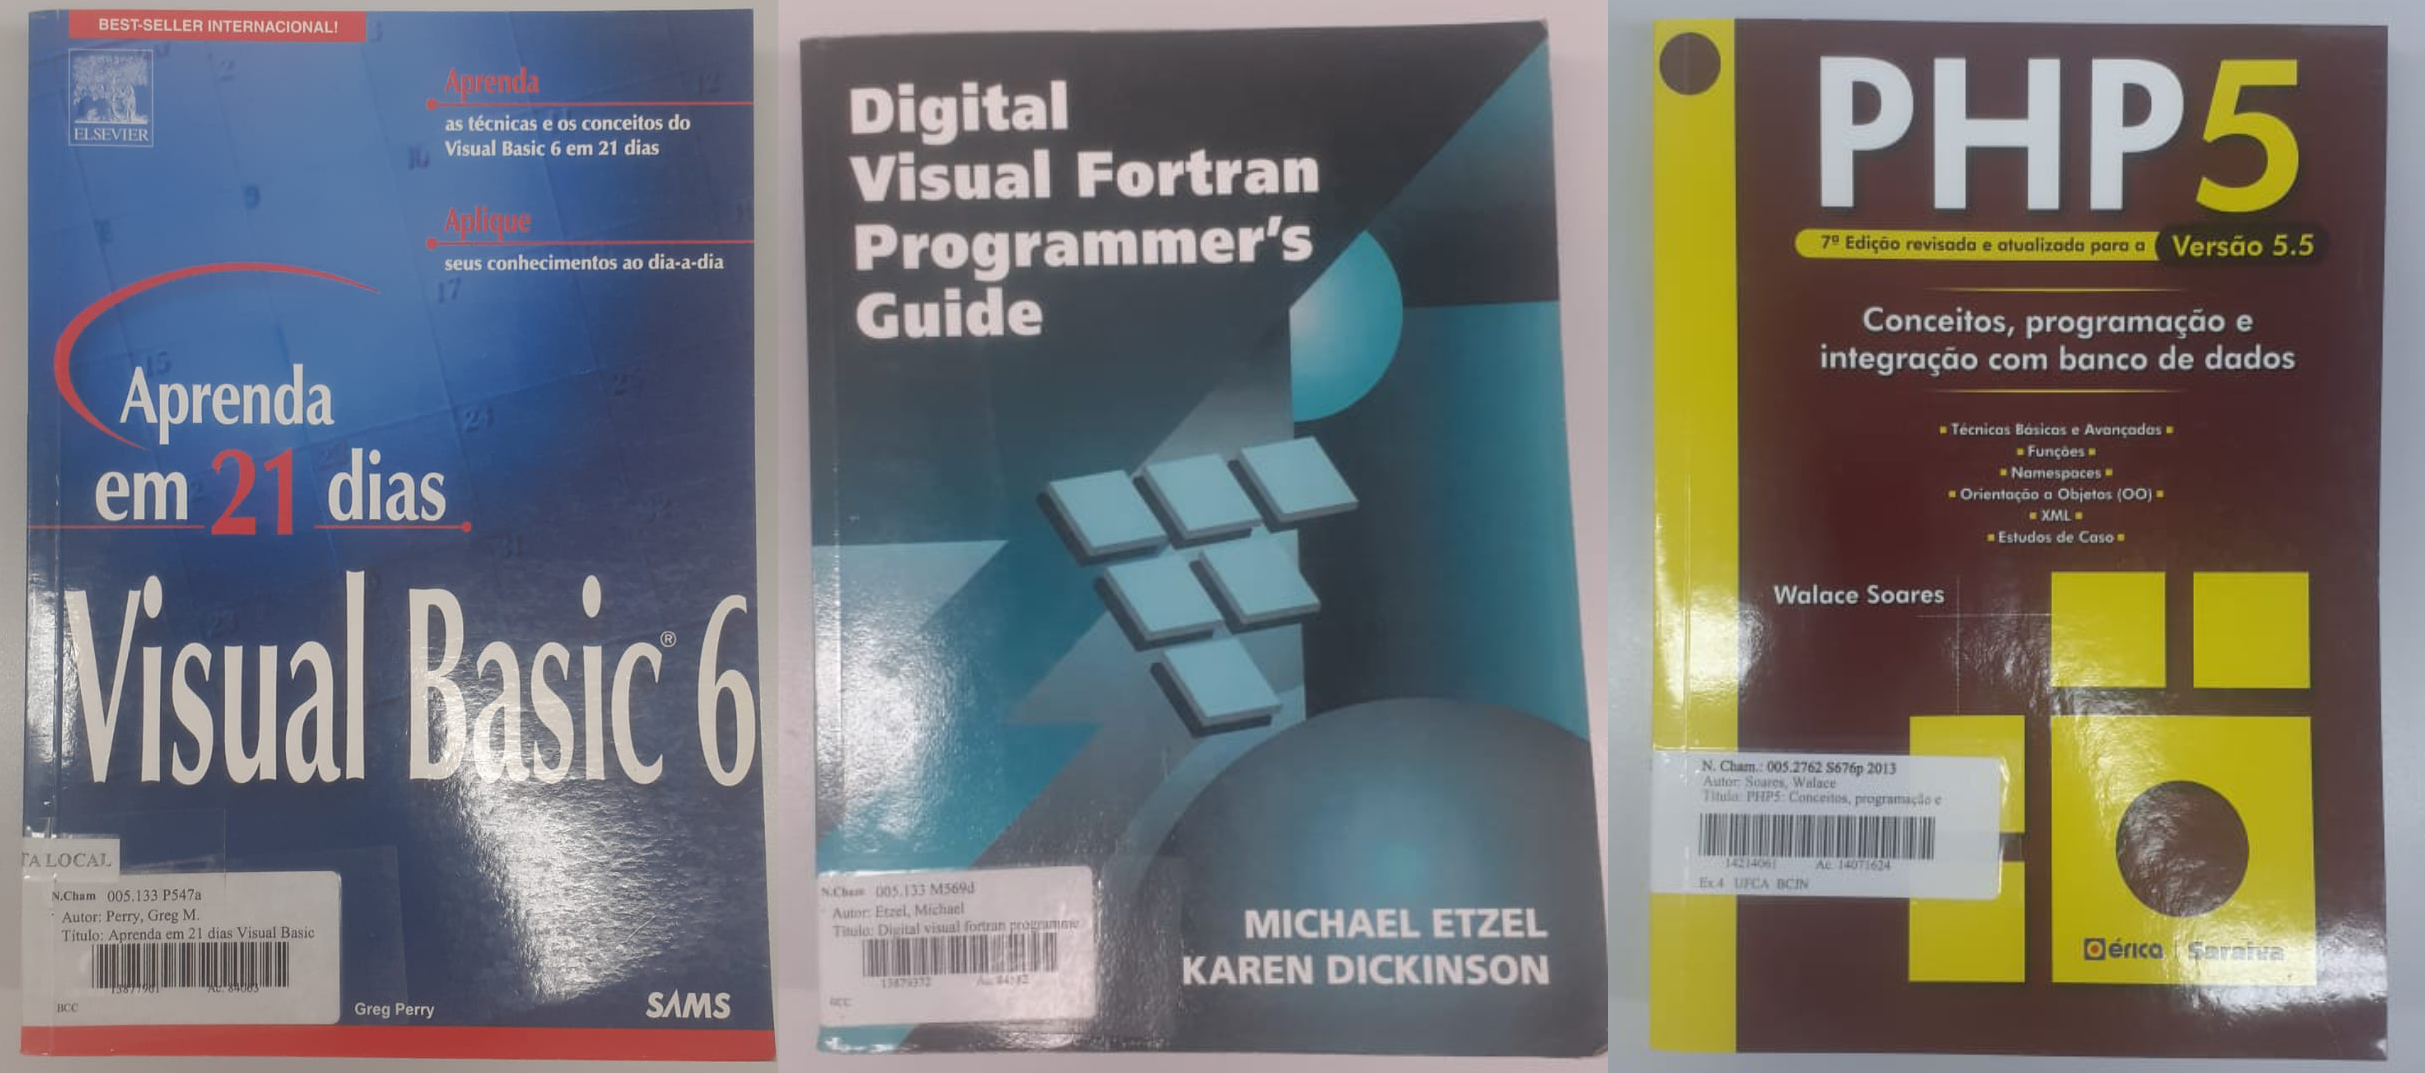
\includegraphics[width=0.6\linewidth]{img/livros.png}
        \caption{Exemplares encontrados no campus Juazeiro do Norte}
        \label{fig:livros}
    \end{figure}
\begin{figure}[t]
        \centering
        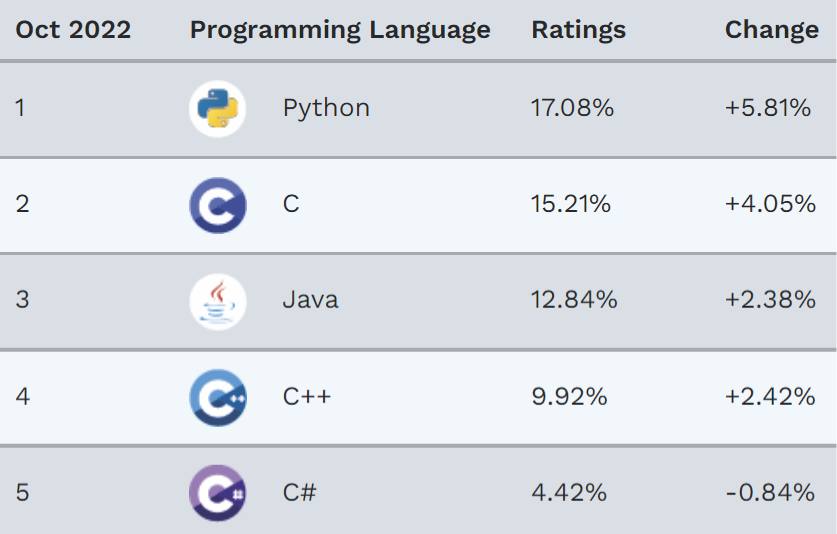
\includegraphics[width=0.6\linewidth]{img/top5.png}
        \caption{Top 5 linguagens mais pesquisadas, segundo a TIOBE}
        \label{fig:top5}
\end{figure}



%%%%%%%%%%%%%%%%%%%%%%%%%%%%%%%%%%%%%%%%%%%%%%%%%%%%%%%%%%%%%%%%%%%%%%%%%%%%%%%%%%%%%%%%%%%%%%%%
%%%%%%%%%%%%%%%%%%%%%%%%%%%%%%%%%%%%%%%%%%%%%%%%%%%%%%%%%%%%%%%%%%%%%%%%%%%%%%%%%%%%%%%%%%%%%%%%
%%%%%%%%%%%%%%%%%%%%%%%%%%%%%%%%%%%%%%%%%%%%%%%%%%%%%%%%%%%%%%%%%%%%%%%%%%%%%%%%%%%%%%%%%%%%%%%%

\pagebreak
\section{Por que Sistemas Embarcados?}
\begin{multicols}{2}
    Ainda que a Ciência da Computação seja uma área infante, comparada com algumas outras, notamos um desenvolvimento exponencial tanto no conhecimento produzido como em suas aplicações na vida cotidiana. Tanembaum \cite{tanenbaum2016structured} discorre brevemente sobre a evolução dos computadores, desde as gigantes máquinas usadas por várias pessoas até minicomputadores familiares operáveis por um só indivíduo. Hoje, presenciamos o ápice até então da miniaturização, no qual cada um de nós possui um dispositivo individual capaz de se conectar a outros, à rede global de informação e, (por que não?) a uma miríade de sensores constantemente captando dados sobre o ambiente.

    O próximo passo nessa evolução, segundo Weiser \cite{weiser1991computer}, é a perfeita integração dos computadores aos objetos mundanos de modo que a capacidade de processamento seja tão natural aos objetos quanto a existência deles próprios. Largos passos nessa direção são dado sempre que um novo produto "inteligente" é adotado pela comunidade. Além disso, diversos fabricantes estão investindo na criação de padrões \cite{build-matter} e protocolos \cite{whatis-lorawan} que simplifiquem a comunicação entre dispositivos de modo que possamos pensar no ambiente em vez dos objetos.

    Também há esforços no desenvolvimento de paradigmas e linguagens de programação capazes de lidar com a grande quantidade de dispositivos e de dados gerados por cada um, a chamada \emph{Ubiquitous Oriented Programming} (UOP) \cite{Garzão_Gonçales_Barbosa_2014}. Isso porque as linguagens tradicionais se mostram como um entrave na criação de novos dispositivos visto não representarem de modo intuitivo nessa situação o problema que se quer solucionar. Este tópico pode ser de interesse para a universidade para futuras produções científicas - envolvendo alunos, se possível.

    Nesse contexto, é importante ressaltar que o desenvolvimento de Sistemas Embarcados não é um fim em si mesmo mas apenas uma ferramenta para que as outras áreas do conhecimento possam oferecer melhores soluções para os problemas cotidianos. Mesmo dentro da universidade, é possível coordenar iniciativas entre o curso de Ciência da Computação e outros cursos ofertados. Dentre eles:

    \begin{itemize}
        \item Engenharia Civil, no planejamento de construções que permitam a instalação de sistemas ubíquos desde a planta, assim como se faz com a rede elétrica.
        \item Medicina e Medicina Veterinária, na monitoração da saúde do paciente com dispositivos vestíveis.
        \item Agronomia, na análise das condições de solo e consumo de água em tempo real.
        \item Libras, pois os alunos com deficiência auditiva podem fornecer \textit{feedback} rápido sobre a acessibilidade dos projetos desenvolvidos.
    \end{itemize}

    Felizmente, a indústria de produtos eletrônicos evolui ao ponto de a maior parte dos processos estar automatizada e a dispor um custo acessível. Mesmo alunos de graduação são capazes de desenvolver produtos de qualidade comercial, uma vez que aprendam as habilidades necessárias. De início, será preciso conhecer:
    
    \begin{itemize}
        \item Programação em linguagem C
        \item Compreensão de microcontroladores dos principais fabricantes (Espressif \cite{esp-devkits}, Microchip \cite{microchip-mcus}, etc)
        \item Eletrônica analógica e digital
        \item Confecção artesanal de PCB com tinta fotossensível
        \item Design de PCB's para industrialização (Altium \cite{altium-designer})
    \end{itemize}

    Devo reconhecer minha perfeita incompetência em todas as cinco habilidades acima e não espero dominá-las em poucas semanas. Não obstante, disponho-me a iniciar um projeto de desenvolvimento de software e hardware e convido colegas interessados e aprende-las durante o processo.
    
\end{multicols}


%%%%%%%%%%%%%%%%%%%%%%%%%%%%%%%%%%%%%%%%%%%%%%%%%%%%%%%%%%%%%%%%%%%%%%%%%%%%%%%%%%%%%%%%%%%%%%%%
%%%%%%%%%%%%%%%%%%%%%%%%%%%%%%%%%%%%%%%%%%%%%%%%%%%%%%%%%%%%%%%%%%%%%%%%%%%%%%%%%%%%%%%%%%%%%%%%
%%%%%%%%%%%%%%%%%%%%%%%%%%%%%%%%%%%%%%%%%%%%%%%%%%%%%%%%%%%%%%%%%%%%%%%%%%%%%%%%%%%%%%%%%%%%%%%%

\pagebreak
\section{Projeto Inicial}
\begin{multicols}{2}

\subsection{Diretrizes}
    Este projeto não tem outros propósitos senão a aquisição de 1) conhecimento técnico, 2) infraestrutura e equipamentos e 3) reconhecimento alunos de outras áreas a fim de que, no futuro, projetos interdisciplinares sejam factíveis.

    Tendo em vista a baixa popularidade do desenvolvimento de Sistemas Embarcados na graduação, acredito que um projeto puramente eletrônico e de programação em baixo nível seria contraprodutivo ao propósito maior. Por isso, proponho que comecemos com algo que seja mais familiar ao recém-ingresso e que, provavelmente, já tenha algum conhecimento prático. Nesta ocasião, usaremos frameworks Web.

    O projeto será executado em duas etapas:
    \begin{enumerate}
        \item Software na Web para prova de conceito. Com ele avaliaremos possíveis mudanças no planejamento e coletaremos avaliações dos usuários. Isso poupará custos de componentes.
        \item Hardware dedicado. Uma vez que se saiba exatamente o que deve ser feito, podemos fazer uma aplicação fixa com o mínimo de gastos.
    \end{enumerate}

\subsection{Solução em Software}
    Notamos que um dos principais meios de interação dos alunos no campus é a prática do Ping Pong. Nesse esporte, cada mesa possui uma fila de pessoas aguardando sua vez de jogar e sempre que alguém quer entrar na fila, pergunta quem é o último e faz uma nota mental pra jogar depois dele.

    Aqui vemos vários problemas. Primeiro, tem apenas uma mesa disponível, obrigando todos a formarem uma única (e longa) fila. Além disso, é um aborrecimento ter que fazer notas mentais sobre a ordem dos jogadores. Imagine a situação: eu quero jogar e pergunto quem é o último na fila, mas ele não responde pois está conversando sendo o penúltimo quem levanta a voz; daí quando este termina de jogar e me aproximo, o último me surpreende com uma conversa desagradável. Não bastasse isso, ordem de jogadores é cíclica, ou seja, quando termino de jogar sou automaticamente posto no final da fila, e o problema anterior se repete.

    A solução é bastante direta: implementar uma forma de dispor por escrito a lista do jogadores e de marcar minha vez. Para isso, planejamos criar um aplicativo Web de fácil uso e baixa latência (Figura \ref{fig:telaInicial}).

    Este aplicativo conterá as seguintes funções:
    \begin{itemize}
        \item Mostrar jogadores da partida atual. Placar é opcional.
        \item Lista de espera em ordem de requisição.
        \item Armazenar dados de cada jogador sobre número de partidas jogadas, de vitórias e de vezes que pediu para jogar e não jogou. Esse último dado será usado pela equipe como forma de avaliar a usabilidade do aplicativo, não necessariamente será visto pelos jogadores.
        \item Recolocar automaticamente os jogadores no fim da fila quando a partida acabar.
    \end{itemize}

    Uma vez que essas funcionalidades estejam implementadas, pode-se implementar outras conforme a demanda. Por exemplo, um ranking usando a quantidade de vitórias de cada jogador bem como um botão para solicitar que a próxima partida seja rankeada.

    Encontrar alguém capaz de criar este aplicativo em poucas semanas não deve ser difícil, já que este nicho é popular atualmente. Além disso, não há custo algum na sua produção exceto pelo tempo do programador e a hospedagem no servidor. Logo, acredito que esta etapa seja concluída muito antes da segunda, permitindo que coletemos dados de usabilidade.

\subsection{Solução em Hardware}
    Observe que o software descrito acima é perfeitamente capaz de, sozinho, resolver o problema na fila de jogadores. Isso nos dá a chance de desenvolver o hardware sem interferir negativamente no decorrer da partida. Se funcionar, ótimo; senão usa-se apenas o aplicativo.

    Esta etapa consistirá na produção de dois componentes: um display conectado à rede capaz de mostrar as mesmas informações do aplicativo, e botões embaixo da mesa pelos quais o jogador possa controlar as informações da partida sem usar o telefone. Com eles, poderemos confirmar que queremos jogar, passar a vez, mudar para o modo de partida em dupla, etc.

    Implementar essas funções pelo software é possível mas desviará a atenção do jogador da mesa para o aparelho, o que pode levar a aborrecimento e prematura obsolência. É preciso fazer testes de campo para confirmar se isso pode de fato ocorrer mas presumo ser possível.

    Seria insensato querer, nesse momento, expandir o escopo deste projeto. Não temos ferramentas, componentes, placas de desenvolvimento, dinheiro, muito menos competência. Adquiri-los levará tempo e esforços consideráveis e dificilmente teremos apoio oficial. Que o leitor esteja ciente disso caso decida participar.

    Por outro lado, se conseguirmos concluir com sucesso este projeto teremos o necessário para iniciar um mais complexo, o qual nos levará a outro, e outro, e assim sucessivamente. Eventualmente, teremos o suficiente para produzir produtos comerciais.
\end{multicols}

\begin{figure}[t]
    \centering
    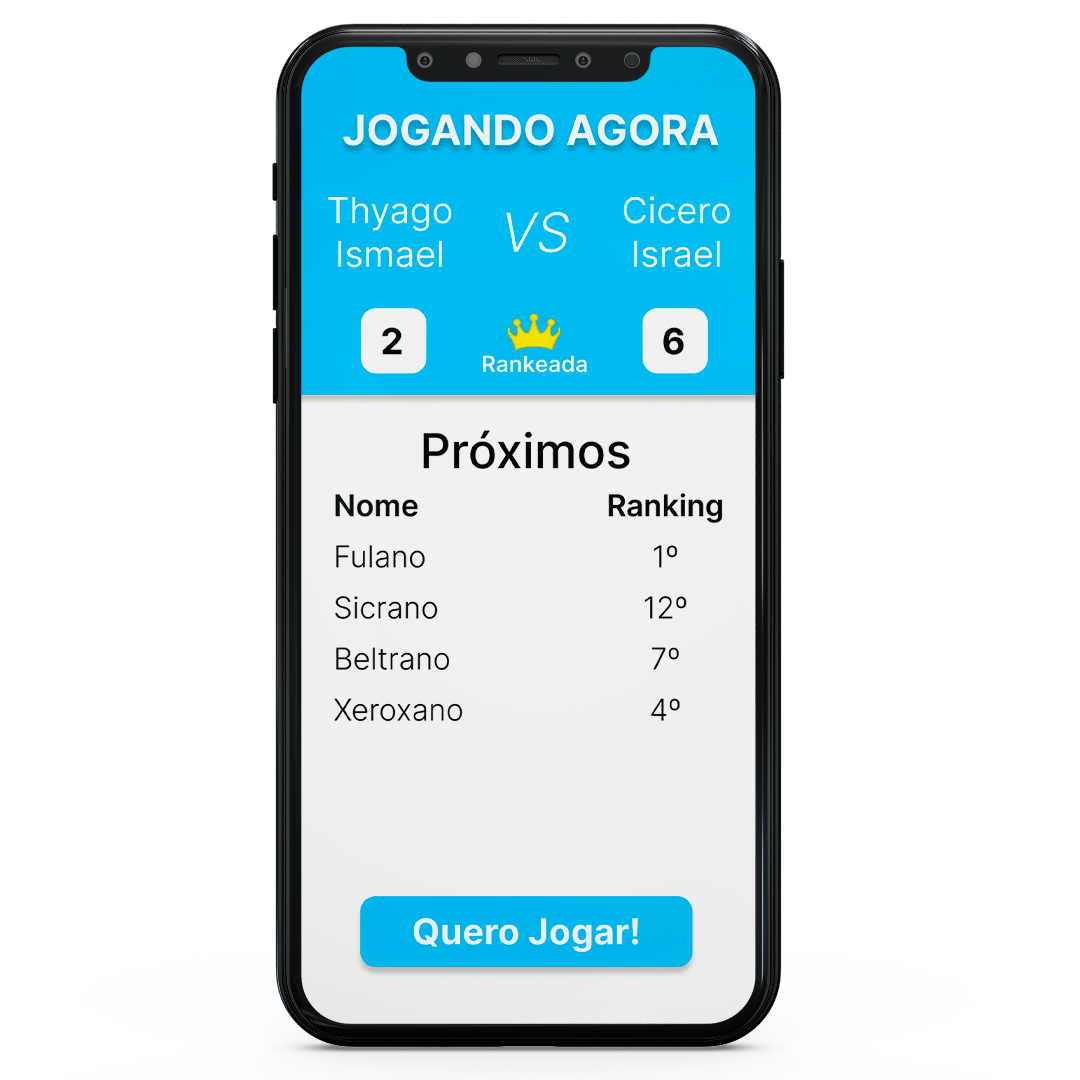
\includegraphics[width=0.6\linewidth]{img/telaInicial.png}
    \caption{Modelo de tela inicial}
    \label{fig:telaInicial}
\end{figure}

%%%%%%%%%%%%%%%%%%%%%%%%%%%%%%%%%%%%%%%%%%%%%%%%%%%%%%%%%%%%%%%%%%%%%%%%%%%%%%%%%%%%%%%%%%%%%%%%
%%%%%%%%%%%%%%%%%%%%%%%%%%%%%%%%%%%%%%%%%%%%%%%%%%%%%%%%%%%%%%%%%%%%%%%%%%%%%%%%%%%%%%%%%%%%%%%%
%%%%%%%%%%%%%%%%%%%%%%%%%%%%%%%%%%%%%%%%%%%%%%%%%%%%%%%%%%%%%%%%%%%%%%%%%%%%%%%%%%%%%%%%%%%%%%%%

\section{Comentários Finais}
\begin{multicols}{2}
    O objetivo deste texto não é substituir as iniciativas existentes na universidade tampouco diminuí-las. Desejo complementá-las apresentando aos colegas discentes mais uma área de possível interesse e construir um local onde possa aplicá-la na prática.

    Hoje, as opções são poucas e de baixo impacto mas com trabalho diário e interesse sério, podemos contribuir positivamente para a comunidade. Os contatos dos alunos atualmente interessados estão escritos na tabela abaixo. Caso o leitor tenha interesse, basta conversar com qualquer um deles.
\end{multicols}


%%%%%%%%%%%%%%%%%%%%%%%%%%%%%%%%%%%%%%%%%%%%%%%%%%%%%%%%%%%%%%%%%%%%%%%%%%%%%%%%%%%%%%%%%%%%%%%%
%%%%%%%%%%%%%%%%%%%%%%%%%%%%%%%%%%%%%%%%%%%%%%%%%%%%%%%%%%%%%%%%%%%%%%%%%%%%%%%%%%%%%%%%%%%%%%%%
%%%%%%%%%%%%%%%%%%%%%%%%%%%%%%%%%%%%%%%%%%%%%%%%%%%%%%%%%%%%%%%%%%%%%%%%%%%%%%%%%%%%%%%%%%%%%%%%


\section{Lista de Alunos Interessados}
\begin{table}[H]
    \centering
    \begin{tabular}{|c|c|c|}
        \hline
        Nome & Matrícula & Email\\ \hline
        Thyago Ismael & 2022005150 & thyago.ismael@aluno.ufca.edu.br\\
        Cicero Israel & 2022002121 & ciceroisrael428@gmail.com \\
        Davi Santos Alexandrino & 2022001812 & davisantos1032@gmail.com \\
        \hline
    \end{tabular}
    \label{tab:lista-interessados}
\end{table}

%%%%%%%%%%%%%%%%%%%%%%%%%%%%%%%%%%%%%%%%%%%%%%%%
%%%%%%%%%%%%%%%%%%%%%%%%%%%%%%%%%%%%%%%%%%%%%%%%
%%%%%%%%%%%%%%%%%%%%%%%%%%%%%%%%%%%%%%%%%%%%%%%%

\vspace{24pt}
\bibliographystyle{plain}
\bibliography{../bibliografia}
\end{document}